\documentclass[a4paper,11pt]{article}

%\usepackage{fullpage}
\usepackage{hyperref}
\usepackage{fixltx2e}
\usepackage{amsmath}
\usepackage{graphicx}
\usepackage{fancyhdr}
\usepackage{listings}



\begin{document}

\title{Natuurlijke taalmodellen en interfaces}
\author{Eszter Fodor \& Sharon Gieske}
\date{\today}
\maketitle

\section*{Question 1}
\textit{grep '\^{}A:'} Deze command zoekt naar een regel die met de empty string (\^{}) begint gevolgd door de letter \textit{A} en dubbelepunt.\\\\
\textit{sed 's/\^{}A: //':} Deze command verwijdert de empty string gevolgd door de letter A en een dubbelepunt \textit{(\^{}A:)} van de door grep gevonden regels. De command \textit{> ovis-trainset.txt} definieert de output file.

\section*{Question 2}
\textit{grep -v '\^{}\$':} Deze command zoekt naar niet lege regels. \textit{-v} betekent dat er juist \textit{niet} naar de gespecificeerde regels moet worden gezocht, in dit geval een lege regel (\^{}\$).\\
\textit{sed 's/\textbackslash s \textbackslash + / \textbackslash n/g':} Verwijdert aan het eind van alle regels de spatie (\textbackslash s) en maakt er een newline van. \\
\textit{uniq -c:} Haalt duplicates uit de input en telt (\textit{-c}) hoeveel keer iedere regel voorkomt. \\
\textit{sort -g -r -k 1:} Sorteert de resultaten aan de hand van de hoeveelheid voorkomens en print deze in reversed volgorde (van het hoogste getal naar het laagste). \textit{-g}: sorteer aan de hand van getallen, \textit{-r}: reverse de volgorde van sorteren, \textit{-k 1}: sorteer op de eerste key.\\

\section*{Question3}
Zipf distribution. ??

\newpage

\section*{Question 4}
Met de volgende opeenvolgende commands kan de word-frequency van austen.txt geplot worden: 
\begin{lstlisting}[frame=single]
less austen.txt | sed 's/\s\+/\n/g' | grep -v '^$' 
	| sort | uniq -c | sort -g -r -k 1 
	> austen-freq.txt
	
gnuplot
gnuplot> plot 'austen-freq.txt' 
	using (log($0)):(log($1))
	gnuplot>set terminal jpeg
gnuplot> set output 'austen.jpg'
gnuplot> plot 'austen-freq.txt' using 
	(log($0)):(log($1))
\end{lstlisting}


\noindent Als output plaatje krijgen we dan:\\
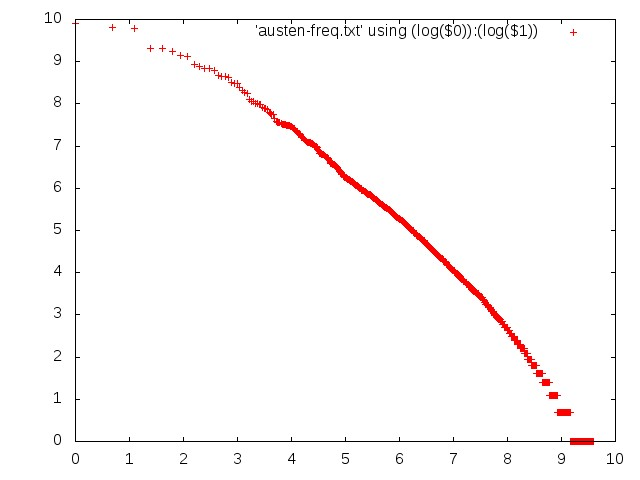
\includegraphics[scale=0.4]{austen.jpg}

\noindent De twee plaatjes van de word-frequencies lijken vrijwel identiek.


\end{document}